\section{States}
This section will explain the internal architecture of the launcher, this is every dependency inside the launcher.
Being able to launch an \girafapp[] as a specific guardian requires the user to interact such that the launcher knows which guardian the user represents.

Authentication was chosen, as each modulated child and guardian contains private data and therefore needs to be protected. QR-codes was chosen as means of authentication, as they provide a level of security.
An alternative to QR-codes could be a \emph{username-password} method, where each user have their own username, with an private password. The system is designed to have the two modes: guardian- and child mode\todo{ref to backlog}. A username-password combination requires the user to remember their credentials, whereas some \autists[] have problems with it. \myQuote{Some \autists[] can have problems remembering a username and password  -  Drazenko Banjak}

QR codes provides a physical way of storing the user credentials and allows for other users to take responsibility of the QR-code, such as a \guardian[] carrying a QR-code of a \autist[].

QR-codes can be scanned by a built-in camera on tablets and can be printed using standard paper and printer equipment. 

QR-codes are copyable, by e.g. a copymachine, and therefore must be kept away from untrusted users, if they should not be used by people for which they were not intended.

To sum up, QR-codes are chosen because of they improve usability, despite of their ability to be copied.\todo{Ulrik, er dette i orden?}



\begin{figure}[h]
	\centering
	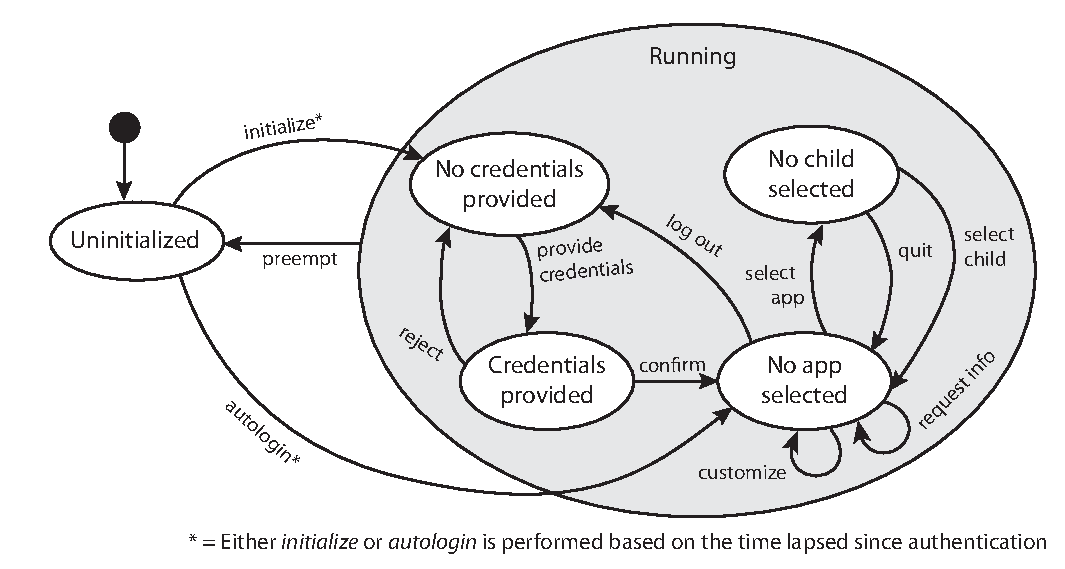
\includegraphics[width=1\textwidth]{gfx/statediagram.pdf}
	\caption{Flow diagram}
	\label{fig:flow_diagram}
\end{figure}

\autoref{fig:flow_diagram} shows the state of the launcher. The first three states handles the distinction between users which are allowed to access the launchable applications, and those who are not. \todo{indsaet ref til der hvor vi fandt ud af at vi skulle have authentication}

